%-*-latex-*-
\tinysidebar{\debug{exercises/{introduction-to-group-theory-2/answer.tex}}}

(a) In $S_5$,
\begin{align*}
\left( (1 \ 4 \ 3)(2 \ 5) \circ (2 \ 3 \ 5) \right)(1) = \left( (1 \ 4 \ 3)(2 \ 5)\right)(1) &= 4 \\
\left( (1 \ 4 \ 3)(2 \ 5) \circ (2 \ 3 \ 5) \right)(2) = \left( (1 \ 4 \ 3)(2 \ 5)\right)(3) &= 1 \\
\left( (1 \ 4 \ 3)(2 \ 5) \circ (2 \ 3 \ 5) \right)(3) = \left( (1 \ 4 \ 3)(2 \ 5)\right)(5) &= 2 \\
\left( (1 \ 4 \ 3)(2 \ 5) \circ (2 \ 3 \ 5) \right)(4) = \left( (1 \ 4 \ 3)(2 \ 5)\right)(4) &= 3 \\
\left( (1 \ 4 \ 3)(2 \ 5) \circ (2 \ 3 \ 5) \right)(5) = \left( (1 \ 4 \ 3)(2 \ 5)\right)(2) &= 5 
\end{align*}
i.e.,
\[
(1 \ 4 \ 3)(2 \ 5) \circ (2 \ 3 \ 5) = (1 \ 4 \ 3 \ 2)(5) = (1 \ 4 \ 3 \ 2) 
\]

(b)
There are $3! = 6$ elements in $S_3$.
The permutation of $S_3$ are
\[
(1), (1 \ \ 2), (1 \ \ 3), (2 \ \ 3),
(1 \ \  2 \ \ 3),
(1 \ \  3 \ \ 2)
\]
The group table of $S_3$ is
%-*-latex-*-
\begin{center}
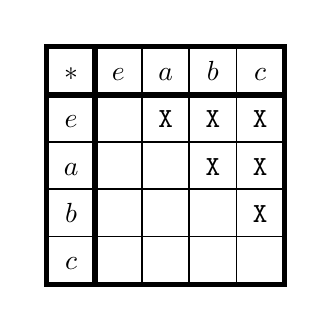
\begin{tikzpicture}

\draw (0.3, -0.3)
  node[draw, line width=0.02cm, , color=black,
       rounded corners=0cm, inner sep=0cm] {

\begin{minipage}[t][0.6cm]{0.6cm}
\mbox{}

\end{minipage}

};\draw (0.3, -0.3) node[color=black] {{\texttt{{\vphantom{$*$$e$$a$$b$$c$X}$*$}}}};\node[anchor=south] at (0.3,0.01) {};\node[anchor=east] at (-0.01,-0.3) {};
\draw (0.3, -0.3)
  node[draw, line width=0.06cm, , color=black,
       rounded corners=0cm, inner sep=0cm] {

\begin{minipage}[t][0.62cm]{0.62cm}
\mbox{}

\end{minipage}

};
\draw (0.8999999999999999, -0.3)
  node[draw, line width=0.02cm, , color=black,
       rounded corners=0cm, inner sep=0cm] {

\begin{minipage}[t][0.6cm]{0.6cm}
\mbox{}

\end{minipage}

};\draw (0.8999999999999999, -0.3) node[color=black] {{\texttt{{\vphantom{$*$$e$$a$$b$$c$X}$e$}}}};
\draw (1.5, -0.3)
  node[draw, line width=0.02cm, , color=black,
       rounded corners=0cm, inner sep=0cm] {

\begin{minipage}[t][0.6cm]{0.6cm}
\mbox{}

\end{minipage}

};\draw (1.5, -0.3) node[color=black] {{\texttt{{\vphantom{$*$$e$$a$$b$$c$X}$a$}}}};
\draw (2.0999999999999996, -0.3)
  node[draw, line width=0.02cm, , color=black,
       rounded corners=0cm, inner sep=0cm] {

\begin{minipage}[t][0.6cm]{0.6cm}
\mbox{}

\end{minipage}

};\draw (2.0999999999999996, -0.3) node[color=black] {{\texttt{{\vphantom{$*$$e$$a$$b$$c$X}$b$}}}};
\draw (2.6999999999999993, -0.3)
  node[draw, line width=0.02cm, , color=black,
       rounded corners=0cm, inner sep=0cm] {

\begin{minipage}[t][0.6cm]{0.6cm}
\mbox{}

\end{minipage}

};\draw (2.6999999999999993, -0.3) node[color=black] {{\texttt{{\vphantom{$*$$e$$a$$b$$c$X}$c$}}}};\node[anchor=south] at (0.8999999999999999,0.01) {};\node[anchor=south] at (1.5,0.01) {};\node[anchor=south] at (2.0999999999999996,0.01) {};\node[anchor=south] at (2.6999999999999993,0.01) {};\node[anchor=east] at (0.59,-0.3) {};
\draw (1.7999999999999996, -0.3)
  node[draw, line width=0.06cm, , color=black,
       rounded corners=0cm, inner sep=0cm] {

\begin{minipage}[t][0.62cm]{2.42cm}
\mbox{}

\end{minipage}

};
\draw (0.3, -0.8999999999999999)
  node[draw, line width=0.02cm, , color=black,
       rounded corners=0cm, inner sep=0cm] {

\begin{minipage}[t][0.6cm]{0.6cm}
\mbox{}

\end{minipage}

};\draw (0.3, -0.8999999999999999) node[color=black] {{\texttt{{\vphantom{$*$$e$$a$$b$$c$X}$e$}}}};
\draw (0.3, -1.4999999999999998)
  node[draw, line width=0.02cm, , color=black,
       rounded corners=0cm, inner sep=0cm] {

\begin{minipage}[t][0.6cm]{0.6cm}
\mbox{}

\end{minipage}

};\draw (0.3, -1.4999999999999998) node[color=black] {{\texttt{{\vphantom{$*$$e$$a$$b$$c$X}$a$}}}};
\draw (0.3, -2.0999999999999996)
  node[draw, line width=0.02cm, , color=black,
       rounded corners=0cm, inner sep=0cm] {

\begin{minipage}[t][0.6cm]{0.6cm}
\mbox{}

\end{minipage}

};\draw (0.3, -2.0999999999999996) node[color=black] {{\texttt{{\vphantom{$*$$e$$a$$b$$c$X}$b$}}}};
\draw (0.3, -2.7)
  node[draw, line width=0.02cm, , color=black,
       rounded corners=0cm, inner sep=0cm] {

\begin{minipage}[t][0.6cm]{0.6cm}
\mbox{}

\end{minipage}

};\draw (0.3, -2.7) node[color=black] {{\texttt{{\vphantom{$*$$e$$a$$b$$c$X}$c$}}}};\node[anchor=south] at (0.3,-0.59) {};\node[anchor=east] at (-0.01,-0.8999999999999999) {};\node[anchor=east] at (-0.01,-1.4999999999999998) {};\node[anchor=east] at (-0.01,-2.0999999999999996) {};\node[anchor=east] at (-0.01,-2.7) {};
\draw (0.3, -1.8)
  node[draw, line width=0.06cm, , color=black,
       rounded corners=0cm, inner sep=0cm] {

\begin{minipage}[t][2.42cm]{0.62cm}
\mbox{}

\end{minipage}

};
\draw (0.8999999999999999, -0.8999999999999999)
  node[draw, line width=0.02cm, , color=black,
       rounded corners=0cm, inner sep=0cm] {

\begin{minipage}[t][0.6cm]{0.6cm}
\mbox{}

\end{minipage}

};\draw (0.8999999999999999, -0.8999999999999999) node[color=black] {{\texttt{{\vphantom{$*$$e$$a$$b$$c$X}}}}};
\draw (1.5, -0.8999999999999999)
  node[draw, line width=0.02cm, , color=black,
       rounded corners=0cm, inner sep=0cm] {

\begin{minipage}[t][0.6cm]{0.6cm}
\mbox{}

\end{minipage}

};\draw (1.5, -0.8999999999999999) node[color=black] {{\texttt{{\vphantom{$*$$e$$a$$b$$c$X}X}}}};
\draw (2.0999999999999996, -0.8999999999999999)
  node[draw, line width=0.02cm, , color=black,
       rounded corners=0cm, inner sep=0cm] {

\begin{minipage}[t][0.6cm]{0.6cm}
\mbox{}

\end{minipage}

};\draw (2.0999999999999996, -0.8999999999999999) node[color=black] {{\texttt{{\vphantom{$*$$e$$a$$b$$c$X}X}}}};
\draw (2.6999999999999993, -0.8999999999999999)
  node[draw, line width=0.02cm, , color=black,
       rounded corners=0cm, inner sep=0cm] {

\begin{minipage}[t][0.6cm]{0.6cm}
\mbox{}

\end{minipage}

};\draw (2.6999999999999993, -0.8999999999999999) node[color=black] {{\texttt{{\vphantom{$*$$e$$a$$b$$c$X}X}}}};
\draw (0.8999999999999999, -1.4999999999999998)
  node[draw, line width=0.02cm, , color=black,
       rounded corners=0cm, inner sep=0cm] {

\begin{minipage}[t][0.6cm]{0.6cm}
\mbox{}

\end{minipage}

};\draw (0.8999999999999999, -1.4999999999999998) node[color=black] {{\texttt{{\vphantom{$*$$e$$a$$b$$c$X}}}}};
\draw (1.5, -1.4999999999999998)
  node[draw, line width=0.02cm, , color=black,
       rounded corners=0cm, inner sep=0cm] {

\begin{minipage}[t][0.6cm]{0.6cm}
\mbox{}

\end{minipage}

};\draw (1.5, -1.4999999999999998) node[color=black] {{\texttt{{\vphantom{$*$$e$$a$$b$$c$X}}}}};
\draw (2.0999999999999996, -1.4999999999999998)
  node[draw, line width=0.02cm, , color=black,
       rounded corners=0cm, inner sep=0cm] {

\begin{minipage}[t][0.6cm]{0.6cm}
\mbox{}

\end{minipage}

};\draw (2.0999999999999996, -1.4999999999999998) node[color=black] {{\texttt{{\vphantom{$*$$e$$a$$b$$c$X}X}}}};
\draw (2.6999999999999993, -1.4999999999999998)
  node[draw, line width=0.02cm, , color=black,
       rounded corners=0cm, inner sep=0cm] {

\begin{minipage}[t][0.6cm]{0.6cm}
\mbox{}

\end{minipage}

};\draw (2.6999999999999993, -1.4999999999999998) node[color=black] {{\texttt{{\vphantom{$*$$e$$a$$b$$c$X}X}}}};
\draw (0.8999999999999999, -2.0999999999999996)
  node[draw, line width=0.02cm, , color=black,
       rounded corners=0cm, inner sep=0cm] {

\begin{minipage}[t][0.6cm]{0.6cm}
\mbox{}

\end{minipage}

};\draw (0.8999999999999999, -2.0999999999999996) node[color=black] {{\texttt{{\vphantom{$*$$e$$a$$b$$c$X}}}}};
\draw (1.5, -2.0999999999999996)
  node[draw, line width=0.02cm, , color=black,
       rounded corners=0cm, inner sep=0cm] {

\begin{minipage}[t][0.6cm]{0.6cm}
\mbox{}

\end{minipage}

};\draw (1.5, -2.0999999999999996) node[color=black] {{\texttt{{\vphantom{$*$$e$$a$$b$$c$X}}}}};
\draw (2.0999999999999996, -2.0999999999999996)
  node[draw, line width=0.02cm, , color=black,
       rounded corners=0cm, inner sep=0cm] {

\begin{minipage}[t][0.6cm]{0.6cm}
\mbox{}

\end{minipage}

};\draw (2.0999999999999996, -2.0999999999999996) node[color=black] {{\texttt{{\vphantom{$*$$e$$a$$b$$c$X}}}}};
\draw (2.6999999999999993, -2.0999999999999996)
  node[draw, line width=0.02cm, , color=black,
       rounded corners=0cm, inner sep=0cm] {

\begin{minipage}[t][0.6cm]{0.6cm}
\mbox{}

\end{minipage}

};\draw (2.6999999999999993, -2.0999999999999996) node[color=black] {{\texttt{{\vphantom{$*$$e$$a$$b$$c$X}X}}}};
\draw (0.8999999999999999, -2.7)
  node[draw, line width=0.02cm, , color=black,
       rounded corners=0cm, inner sep=0cm] {

\begin{minipage}[t][0.6cm]{0.6cm}
\mbox{}

\end{minipage}

};\draw (0.8999999999999999, -2.7) node[color=black] {{\texttt{{\vphantom{$*$$e$$a$$b$$c$X}}}}};
\draw (1.5, -2.7)
  node[draw, line width=0.02cm, , color=black,
       rounded corners=0cm, inner sep=0cm] {

\begin{minipage}[t][0.6cm]{0.6cm}
\mbox{}

\end{minipage}

};\draw (1.5, -2.7) node[color=black] {{\texttt{{\vphantom{$*$$e$$a$$b$$c$X}}}}};
\draw (2.0999999999999996, -2.7)
  node[draw, line width=0.02cm, , color=black,
       rounded corners=0cm, inner sep=0cm] {

\begin{minipage}[t][0.6cm]{0.6cm}
\mbox{}

\end{minipage}

};\draw (2.0999999999999996, -2.7) node[color=black] {{\texttt{{\vphantom{$*$$e$$a$$b$$c$X}}}}};
\draw (2.6999999999999993, -2.7)
  node[draw, line width=0.02cm, , color=black,
       rounded corners=0cm, inner sep=0cm] {

\begin{minipage}[t][0.6cm]{0.6cm}
\mbox{}

\end{minipage}

};\draw (2.6999999999999993, -2.7) node[color=black] {{\texttt{{\vphantom{$*$$e$$a$$b$$c$X}}}}};\node[anchor=south] at (0.8999999999999999,-0.59) {};\node[anchor=south] at (1.5,-0.59) {};\node[anchor=south] at (2.0999999999999996,-0.59) {};\node[anchor=south] at (2.6999999999999993,-0.59) {};\node[anchor=east] at (0.59,-0.8999999999999999) {};\node[anchor=east] at (0.59,-1.4999999999999998) {};\node[anchor=east] at (0.59,-2.0999999999999996) {};\node[anchor=east] at (0.59,-2.7) {};
\draw (1.7999999999999996, -1.8)
  node[draw, line width=0.06cm, , color=black,
       rounded corners=0cm, inner sep=0cm] {

\begin{minipage}[t][2.42cm]{2.42cm}
\mbox{}

\end{minipage}

};
\end{tikzpicture}

\end{center}



(c) From the group table, when I look at the entry at row 2, column 1
and the entry at row 1, column 2, I see two different values.
(For me, the row and column indices begin with $0$ and not $1$).
\begin{align*}
\text{row 2, column 1} &: (1 \ 2) \circ (1 \ 3) = (1 \ 3 \ 2) \\
\text{row 1, column 2} &: (1 \ 3) \circ (1 \ 2) = (1 \ 2 \ 3) 
\end{align*}
Therefore $S_3$ is non-abelian.
\qed
